\section{Natural language processing}
\label{sec:nlp}

% inroduction and why interesting
Natural language processing (NLP) aims to read text and extract meaningful information from it.
One deviation from this definition is natural language generation, where text is generated.
Note that this differs from interpretation of text and then returning some pre-defined piece of text.
The difficulty in NLP is that humans have evolved to use a concise way of communication which makes use of knowledge from the world and context.
For example, the response to ``I want more money.'' depends on whether the sentence is uttered by a child or employee.
A perfect NLP system would need artificial general intelligence or is `AI-complete'.
Current artificial intelligence systems ``demonstrate intelligence in only one or another specialised area''~\citep{pennachin2007contemporary}, so called `narrow AI'.
This makes it an field which is far from solved.

% tasks
The field is divided in tasks.
Some well-known tasks are:
\begin{itemize}
    \item Translating texts or \textbf{machine translation}.
    \item \textbf{Question answering} which is NLP on question sentences only.
    \item Classifying words or parts of sentences is done by \textbf{part-of-speech tagging} and \textbf{named-entity recognition}.
    \item \textbf{Optical character recognition} can use NLP knowledge to improve accuracy.
    \item Finding co-references like ``The \underline{house} is white, and \underline{it} is located on a hill.'' is done using \textbf{coreference resolution}.
    \item NLP is not limited to text, because it includes \textbf{speech recognition} which transforms speech to text.
\end{itemize}

\subsection{Language model}
\label{subsec:language_model}
To be able to explain more complex neural network architectures we first take a look at a simple language model.
Language models try to capture the grammar of a language.
Capturing grammar can be done by using probabilities for sentences or probabilities of upcoming words given a part of a sentence.
It is based on the assumption that grammatically correct sentences occur more often than incorrect sentences.
The following three tasks demonstrate the usefulness of probabilities.
\begin{center}
    \begin{tabular}{l l}
        Spell correction & $P(\text{my car broke}) > P(\text{my car boke})$\\
        Machine translation & $P(\text{the green house}) > P(\text{the house green})$\\
        Speech recognition & $P(\text{the red car}) > P(\text{she read ar})$
    \end{tabular}\\
\end{center}

A simple approach is to use counters to calculate the sentence probabilities.
This makes use of the chain rule.
Let $W$ denote a sentence, or equivalently, sequence of words.
For the probability of the sentence we have $P(W) = P(w_1, w_2, \ldots, w_n)$.
The probability of the upcoming word $w_i$ is $P(w_i) = P(w_i \: | \: w_1, w_2, \ldots, w_{i-1})$.
Using the chain rule we can, for three variables, state that $P(w_3, w_2, w_1) = P(w_3 \: | \: w_2, w_1) \cdot P(w_2 \: | \: w_1) \cdot P(w_1)$.
This pattern scales to any number of variables.
To get the probability for the sentence `the car broke` we rewrite it as follows.
\[ P(\text{the car broke}) = P(\text{the}) \cdot P(\text{car} \: | \: \text{the}) \cdot P(\text{broke} \: | \: \text{the car}) \]
Each term can be rewritten to a combination of counters, for example: $P(\text{broke} \: | \: \text{the car}) = \textsc{count}(\text{the car}) \: / \: \textsc{count}(\text{broke})$.
This does not scale well.
The counters for each word and each pair of words are feasible.
However, when doing this for long sentences the number of counters to keep track of becomes too large.

To reduce the number of counters an approximation defined by Markov is used.
Markov states that only looking at a fixed number of previous words gives an approximation.
Considering only one previous word for our example we get the following.
\[ P(\text{broke} \: | \: \text{the car}) \approx P(\text{broke} \: | \: \text{car}) \]
This is called the bigram model.
When using this to generate sentences it becomes clear that bigrams do not have enough information.
Take the generated sentence ``I cannot betray a trust of them.''~\citep{langkilde1998practical}.
Each pair of sequential words is correct, while the sentence as a whole is not.
This simplification of looking at a fixed number of previous words is called n-grams.
Although n-grams offer good performance for certain cases they are in practise not able to capture long-distance dependencies in texts.

\subsection{Machine translation}
\label{subsec:mt}
% introduction
Machine translation became known to the public by introduction of Google Translate in 2006.
The system was statistical (as explained in section~\ref{subsec:language_model}) and not rule-based.
Rule-based means formulating linguistic rules which is ``a difficult job and requires a linguistically trained staff''~\citep{sumita1991experiments}.
In an attempt to visualise the progress made in the field we consider the `one sentence benchmark' by~\citet{manning2017lectures}.
This benchmark contains one Chinese to English example which is compared with Google Translate output.
The correct translation for the example is:\\

In 1519, six hundred Spaniards landed in Mexico to conquer the Aztec Empire with a population of a few million.
They lost two thirds of their soldiers in the first clash.\\

Google Translate returned the following translations.

\begin{description}
    \item[2009] 1519 600 Spaniards landed in Mexico, millions of people to conquer the Aztec empire, the first two-thirds of soldiers against their loss.
    \item[2011] 1519 600 Spaniards landed in Mexico, millions of people to conquer the Aztec empire, the initial loss of soldiers, two thirds of their encounters.
    \item[2013] 1519 600 Spaniards landed in Mexico to conquer the Aztec empire, hundreds of millions of people, the initial confrontation loss of soldiers two-thirds.
    \item[2014-2016] 1519 600 Spaniards landed in Mexico, millions of people to conquer the Aztec empire, the first two-thirds of the loss of soldiers they clash.
    \item[2017] In 1519, 600 Spaniards landed in Mexico, to conquer the millions of people of the Aztec empire, the first confrontation they killed two-thirds.
\end{description}

% alignment
One important concept in machine translation is alignment.
Alignment refers to the fact that words in different languages tend to be aligned.
Consider the sentences

\begin{center}
    ``\underline{well i think if we} can make it \underline{at eight on both days}''
\end{center}
and
\begin{center}
    ``\underline{ja ich denke wenn wir} das hinkriegen \underline{an beiden tagen acht uhr}''.
\end{center}
The first five words of the sentences are perfectly aligned.
The last five words of the sentences are not.
Alignment is visualised in figure~\ref{fig:alignment}.
Non-perfect alignment can also be observed from the fact that the number of words in English sentence is higher.

\begin{figure}[htbp]
    \begin{center}
        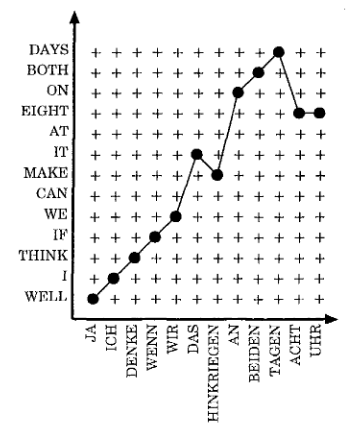
\includegraphics[scale=0.4]{figures/alignment.png}
        \vspace*{-2mm}
    \end{center}
    \caption{Word alignment for a German-English sentence pair~\cite[Figure 1]{vogel1996hmm}.}
    \label{fig:alignment}
\end{figure}